\documentclass{msuposter}

%%%%%%%%%%%%%%%%%%%%%%%%%%%%%%%%%%%%%%%%%%%%%%%%%%%
%% Packages
%%%%%%%%%%%%%%%%%%%%%%%%%%%%%%%%%%%%%%%%%%%%%%%%%%%
\usepackage{lipsum}
\usepackage{tikz,wrapfig}
\usepackage{bm,color}
\usepackage{marginnote}
\usepackage{amsmath}
\usepackage{amssymb}
\usepackage{mathtools}
\usepackage{multicol}
\usepackage{nicefrac}
\usepackage{cleveref}
\usepackage{algorithm}
\usepackage{algpseudocode}
\usepackage{float}
\usepackage[numbers,sort&compress]{natbib}
\usepackage[dvipsnames,svgnames]{xcolor}
\usepackage{booktabs}\let\cline\cmidrule

%% Hyperparameters
\newcommand\myshade{85}
\colorlet{mylinkcolor}{violet}
\colorlet{mycitecolor}{YellowOrange}
\colorlet{myurlcolor}{Aquamarine}
\hypersetup{
    colorlinks=true,
    linkcolor  = mylinkcolor!\myshade!black,
    citecolor  = mycitecolor!\myshade!black,
    urlcolor   = myurlcolor!\myshade!black,
}
%%%%%%%%%%%%%%%%%%%%%%%%%%%%%%%%%%%%%%%%%%%%%%%%%%%
%% Macros
%%%%%%%%%%%%%%%%%%%%%%%%%%%%%%%%%%%%%%%%%%%%%%%%%%%
%% Miscellaneous
\newcommand{\colwidth}{0.32\linewidth}
%% Math commands 
\newcommand{\R}{\mathbb{R}} % real numbers
\newcommand{\N}{\mathcal{N}} % Normal distribution
\newcommand{\id}{\mathbf{I}} % identify matrix
\newcommand{\eqdef}{:=}
%% Parameters
\newcommand{\p}{{\color{ForestGreen}\mathbf{p}}}
\newcommand{\pstar}{\p^*}
\newcommand{\phat}{\hat{\p}_{\mathrm{MAP}}}
%% On the continuum
\renewcommand{\u}{\boldsymbol{u}}
\renewcommand{\t}{t}
\newcommand{\noise}{\boldsymbol{\varepsilon}}
%% Functions
\newcommand{\testFun}{\boldsymbol{\varphi}}
\newcommand{\f}{\boldsymbol{f}}
\newcommand{\F}{\boldsymbol{F}}
\newcommand{\G}{\boldsymbol{G}}
\newcommand{\g}{\boldsymbol{g}}
\renewcommand{\b}{\mathbf{b}}
\renewcommand{\r}{\mathbf{r}}
\renewcommand{\S}{\mathbf{S}}
\newcommand{\loglikelihood}{\ell}
%% Discrete analogues
\newcommand{\udisc}{\mathbf{u}}
\newcommand{\Udisc}{\mathbf{U}}
\newcommand{\tdisc}{\mathbf{t}}
\newcommand{\TestFundisc}{\boldsymbol{\Phi}}
\newcommand{\Noisedisc}{\mathbf{\mathcal{E}}}
\newcommand{\Q}{\mathbf{Q}}
%% Operators
\DeclareMathOperator{\logdet}{logdet}
\DeclareMathOperator{\argmin}{argmin}
\DeclareMathOperator{\vecOp}{vec}

%%%%%%%%%%%%%%%%%%%%%%%%%%%%%%%%%%%%%%%%%%%%%%%%%%%
%% Start Document
%%%%%%%%%%%%%%%%%%%%%%%%%%%%%%%%%%%%%%%%%%%%%%%%%%%

%% Title Information
\title{Bayesian weak form Estimation of Nonlinear Dynamics (BENDy)}
\author{N.~Rummel, S.~Becker, D.M.~Bortz, V.~Dukic}
\institute{Department of Applied Mathematics, University of Colorado Boulder
% ,\inst{2} Los Alamos National Laboratory
}

\begin{document}
\begin{frame}{}
\begin{columns}[t]
%%%%%%%%%%%%%%%%%%%%%%%%%%%%%%%%%%%%%%%%%%%%%%%%%%%
%% Left Column
%%%%%%%%%%%%%%%%%%%%%%%%%%%%%%%%%%%%%%%%%%%%%%%%%%%
\begin{column}{\colwidth}
\begin{block}{Contributions}
    \begin{itemize}
        \item Extended prior work \citep{BortzMessengerDukic2023BullMathBiol} to \alert{nonlinear-in-parameters} systems.
        \item Formulated analytic expressions for an approximate likelihood and its derivatives.
        \item Implemented efficient and application friendly Julia \citep{BezansonEdelmanKarpinskiEtAl2017SIAMRev} code.
        \item Accommodated more general noise distributions.
        \item Extended to a Bayesian framework with automatic \alert{objective priors}.
        \item Guaranteed \alert{consistency} of the BENDy estimator.
    \end{itemize}
\end{block}

\begin{block}{Weak Form Parameter Estimation}
    \textbf{Goal:}  \alert{Estimate the unknown parameters} $\p\in \mathbb{R}^J$.

    Given a (possibly \emph{nonlinear}) system of differential equations  
    % \small
    \begin{equation} \label{eq:ode-strong}
        \dot{\u} = \f(\p,\u,\t)
    \end{equation}
    \normalfont
    where $\f: \R^J \times \R^D \times \R \rightarrow \R^D$,
    $\u \in \R^D$ and $t\in [0,T]$.

    Transform \cref{eq:ode-strong} to its \alert{weak form} by taking the inner product of both sides with a test function $\testFun$ along each dimension
    % \small
    \begin{equation} \label{eq:ode-weak}
        -\langle \dot{\testFun}, \u\rangle = \langle \testFun, \f(\p, \u, \t)\rangle%, \quad \forall \testFun \in \mathcal{C}_0^\infty([0,T])
    \end{equation}
    \normalfont
    Assume access to $M+1$ observations
    % \small
    % \begin{equation}\label{eq:data}
        $\{(\mathrm{t}_m, \Udisc_m)\}_{m=0}^M$
    % \end{equation}
    % \normalfont
    where the data has been corrupted by noise $\noise_m \stackrel{iid}{\sim} \N(\mathbf{0},\Sigma)$.
    \begin{table}
    \begin{tabular}{lc}
        \textbf{Distribution} & \textbf{Data Description}\\
        \midrule
        Additive Gaussian & $\Udisc_m = \udisc_m + \noise_m$ \\
        Multiplicative LogNormal & $\Udisc_m = \udisc_m \exp(\noise_m)$
    \end{tabular}
    \end{table}
\end{block}

\begin{block}{Discritization}
    Selecting specific test functions $\{\testFun\}_{k=1}^K$, the inner products can be approximated through quadrature.
    % \small
    \begin{equation}\label{eq:weakFormDisc}
        - \dot{\TestFundisc} \Q \Udisc \approx \TestFundisc \Q \F(\Udisc,\tdisc,\p) .
    \end{equation}
    \normalfont
    where the following are defined for convenience:
    % \small 
    \begin{table}
    \begin{tabular}{ll}
        % \textbf{Variable} & \textbf{}
        Test Function Matrix & $\TestFundisc \in \R^{K\times (M+1)}$ \\
        Quadrature Matrix &$\Q\in \R^{(M+1)\times (M+1)}$\\
        Observation Matrix & $\Udisc \in \R^{(M+1)\times D}$ \\
        Matrix-valued Function & $\F: \R^{(M+1)\times D}\times \R^{M+1} \times \R^J \rightarrow \R^{(M+1)\times D}$ 
    \end{tabular}
    \end{table}
    \normalfont
\end{block}
\end{column}

%%%%%%%%%%%%%%%%%%%%%%%%%%%%%%%%%%%%%%%%%%%%%%%%%%%
%% Middle Column
%%%%%%%%%%%%%%%%%%%%%%%%%%%%%%%%%%%%%%%%%%%%%%%%%%%

\begin{column}{\colwidth}
\begin{block}{Approximate Distribution}
    In expectation, the \alert{weak residual} should be small 
    \small
    \begin{equation}\label{eq:wres}
        \mathbf{0} \approx \r(\p) := \vecOp\left[\dot{\TestFundisc} \Q \F(\Udisc,\tdisc,\p) + \TestFundisc \Q \Udisc\right] \in \R^{KD}
    \end{equation}
    \normalfont
    when $\p \approx \p^*$. Notice, $\r(\p^*) \neq \mathbf{0}$ because 
    \begin{itemize}
        \item Inner products are \emph{approximated} through quadrature.
        \item Data $\Udisc$ is noisy.
    \end{itemize}

    Through a \emph{linearization} with respect to $\u$ about the data $\Udisc$, one can obtain the \alert{approximate distribution} of the weak residual
    \small
    \begin{equation}\label{eq:weakResDist}
        \S(\p)^{-\nicefrac{1}{2}} \r(\p) \stackrel{approx}{\sim} \N(\mathbf{0}, \id)
    \end{equation}
    \normalfont
    where an analytic expression for $\S$ follows from the linearization and the noise distribution, see \citep{RummelMessengerBeckerEtAl2025arXiv250208881}.
    % Moving all the parameters to the right hand side, we can define an expression for the \emph{weak residual} 
    % \begin{equation}\label{eq:wres}
    %     \mathbf{r}(\p) := \vecOp\left[\dot{\TestFundisc} \Q \F(\Udisc,\tdisc,\p) + \TestFundisc \Q \Udisc\right] \in \R^{(M+1)D}
    % \end{equation}
    % where $\vecOp$ vectorizes the matrix expression on the right hand side of \cref{eq:weakFormDisc}. Because the quadrature  \emph{approximates} the underlying integrals, and the data has been \emph{corrupted by noise}, one can expect $r$ to be \emph{small}, albeit not zero,  when evaluated at the true parameters.
\end{block}


\begin{block}{Maximum a Posteriori Estimator}
    Often a \alert{prior} for the parameters $\p \sim \Pi$ is known. Alternatively, one can utilize an \emph{objective prior} \citep{JordanMcLoughlin,Robert2007,ChoiRamamoorthi2008InstituteofMathematicalStatisticsCollections}. 
    %Priors encode information known from experts or context such as \emph{constraints}.

    The approximate negative log-\alert{posterior} is proportional to
    \small
    \begin{equation}\label{eq:posterior}
        \ell(\p) \propto \logdet\bigl(\S(\p)\bigr) + \r(\p)^\top \S(\p)^{-1}\r(\p) + \pi(\p).
    \end{equation}
    \normalfont
% \end{block}
% \begin{block}{Optimization}
    The unknown parameters can be obtained via \alert{optimization}
    % \small
    \begin{equation}\label{eq:opt}
        \phat = \underset{\p}{\argmin}\Bigl( \ell(\p)\Bigr).
    \end{equation}\vspace{-3mm}
\end{block}

\begin{block}{Consistency}
    Recall, the \emph{Gaussian approximation} is obtained via a \emph{linearization} with respect to $\u$; this leads to \alert{bias}, even when data is dense
    \small
    \begin{equation}\label{eq:bias}
        \lim_{M \rightarrow \infty}\mathbb{E}[\phat] \neq \pstar.
    \end{equation}
    \normalfont
    To address this, correct by using more terms in the expansion
    \small
    \begin{equation}\label{eq:corrector}
    \begin{gathered}
        \mathbf{c}(\p) = (\TestFundisc \Q \nabla_p \F(\tdisc, \Udisc, \p))^\dagger \vecOp\left[\sum_{\alpha=2}^{\alpha_{\mathrm{trunc}}} \frac{1}{\alpha!}\TestFundisc \Q \mathbb{E}\bigl[\nabla_{\u}^\alpha \F(\tdisc, \Udisc, \p)  \times_1 \Noisedisc \cdots \times_\alpha \Noisedisc  \bigr]\right],\\
        \hat{\p}_{\mathrm{cor}} = 
        \hat{\p}_{\mathrm{MAP}} - \mathbf{c}(\hat{\p}_{\mathrm{MAP}}).
    \end{gathered}
    \end{equation}
    \normalfont
    \Cref{eq:corrector} can be approximated via analytic expressions for $\nabla_{\u}^\alpha \F$ and known centered moments for Gaussians or by sampling. 

    In a neighborhood of $\pstar$, \emph{consistency} is obtained 
    % \small
    \begin{equation}\label{eq:consistency}
        \lim_{M\rightarrow \infty} \mathbb{E}[\hat{\p}_{\mathrm{cor}} ]= \p^*.
    \end{equation}\vspace{-3mm}
    % To address this, solve a \alert{nonlinear system} in a post process 
    % \begin{equation}\label{eq:postProc}
    %     \min_{\p} \Bigl\|\bigl(\TestFundisc \Q \nabla_\p F(\tdisc, \Udisc, \p)\bigr)^{\dagger} \r(\tdisc, \Udisc, \p) \Bigr\|_2.
    % \end{equation}
    % In a neighborhood of the true state, the Johnson–Lindenstrauss lemma guarantees the inverse of linearization about $p$ can be used 
    % \begin{equation}\label{eq:jl-lemma}
    % (\TestFundisc \Q \nabla_\p F(\tdisc, \Udisc^*, \p^*))^\dagger \approx \TestFundisc \Q \nabla_\p F(\tdisc, \Udisc, \p)^\dagger
    % \end{equation}
    % \begin{algorithm}[H] % you need to use the float [H] flag to force this in the minipage
    % \small
    % \begin{center} \begin{minipage}{0.9\linewidth} \begin{algorithmic}
    % \Procedure{biasCorrection}{}%$\A[\cdot], \b, \x_0; k_{\max}, \epsilon_{\mathrm{kkt}}$}
    %     \State Set $\p^{(0)} = \phat, \mathbf{c}^{(0)} := \TestFundisc \Q \nabla_{\p} \F(\t,\Udisc,\p^\alpha)^{-1} \mathbf{c}(\p^{(0)})$
    %     \For{$n \gets 1:n_{\mathrm{max}}$}
    %         \State $\p^{n} \gets \phat - \mathbf{c}^{(n-1)}$
    %         \If{$\|\p^{(n)} - \p^{(n-1)}\| \ll \varepsilon_{\mathrm{tol}}$} 
    %             \State \Return $\p^{(n)}$
    %         \EndIf
    %         \State $c^{(n)} \gets \nabla_{\p} \F(\t,\Udisc,\p^{(n)})^{-1} \mathbf{c}(\p^{(n)})$
    %     \EndFor
    %     \State \Return $\p^{(n)}$
    % \EndProcedure
    % \end{algorithmic} \end{minipage} \end{center}
    % \end{algorithm}
\end{block} 

\end{column}


%%%%%%%%%%%%%%%%%%%%%%%%%%%%%%%%%%%%%%%%%%%%%%%%%%%
%% Right Column
%%%%%%%%%%%%%%%%%%%%%%%%%%%%%%%%%%%%%%%%%%%%%%%%%%%
\begin{column}{\colwidth}



\begin{exampleblock}{Example: Logistic Growth}
    Consider the ordinary differential equation
    % \small
    \begin{equation} \label{eq:logisticGrowth}
            \dot{u} = p_1 u - p_2 u^2
    \end{equation}
    where $t \in [0,10]$ and $\pstar = [2.25, 7.0]^\top$.
    \normalfont
    Data is observed on a uniform grid $\{(m\Delta t, \mathrm{u}_m)\}_{m=0}^M$ corrupted by \alert{multiplicative LogNormal} noise. 
    \begin{figure}[H]
        \centering
        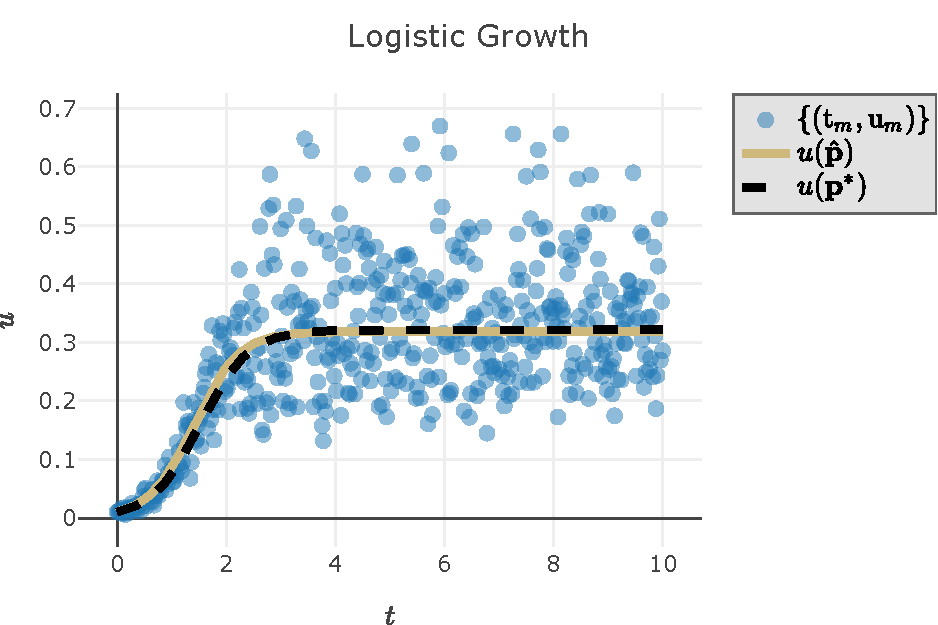
\includegraphics[width=0.75\linewidth]{figures/LogisticGrowth_TrajectoryWithData.pdf}
        % \caption{The true parameters are near the mode of the priors, but not exactly. Information from the ODE is necessary to better estimate parameters.}
        \label{fig:LogisticGrowth-oneDimPriors}
    \end{figure}
    Given the \alert{priors}
    % \small
    % \begin{center}
        ${\color{ForestGreen} p}_1 \sim 2(\beta(2,5) +0.8)$ and ${\color{ForestGreen} p}_2 \sim \text{Fr\'echet}(\alpha=3, \theta=5.503)$,
    % \end{center}
    \normalfont
    one can now estimate  $\p$ with \cref{eq:opt} and \cref{eq:corrector}. 
    \begin{figure}[H]
        \centering
        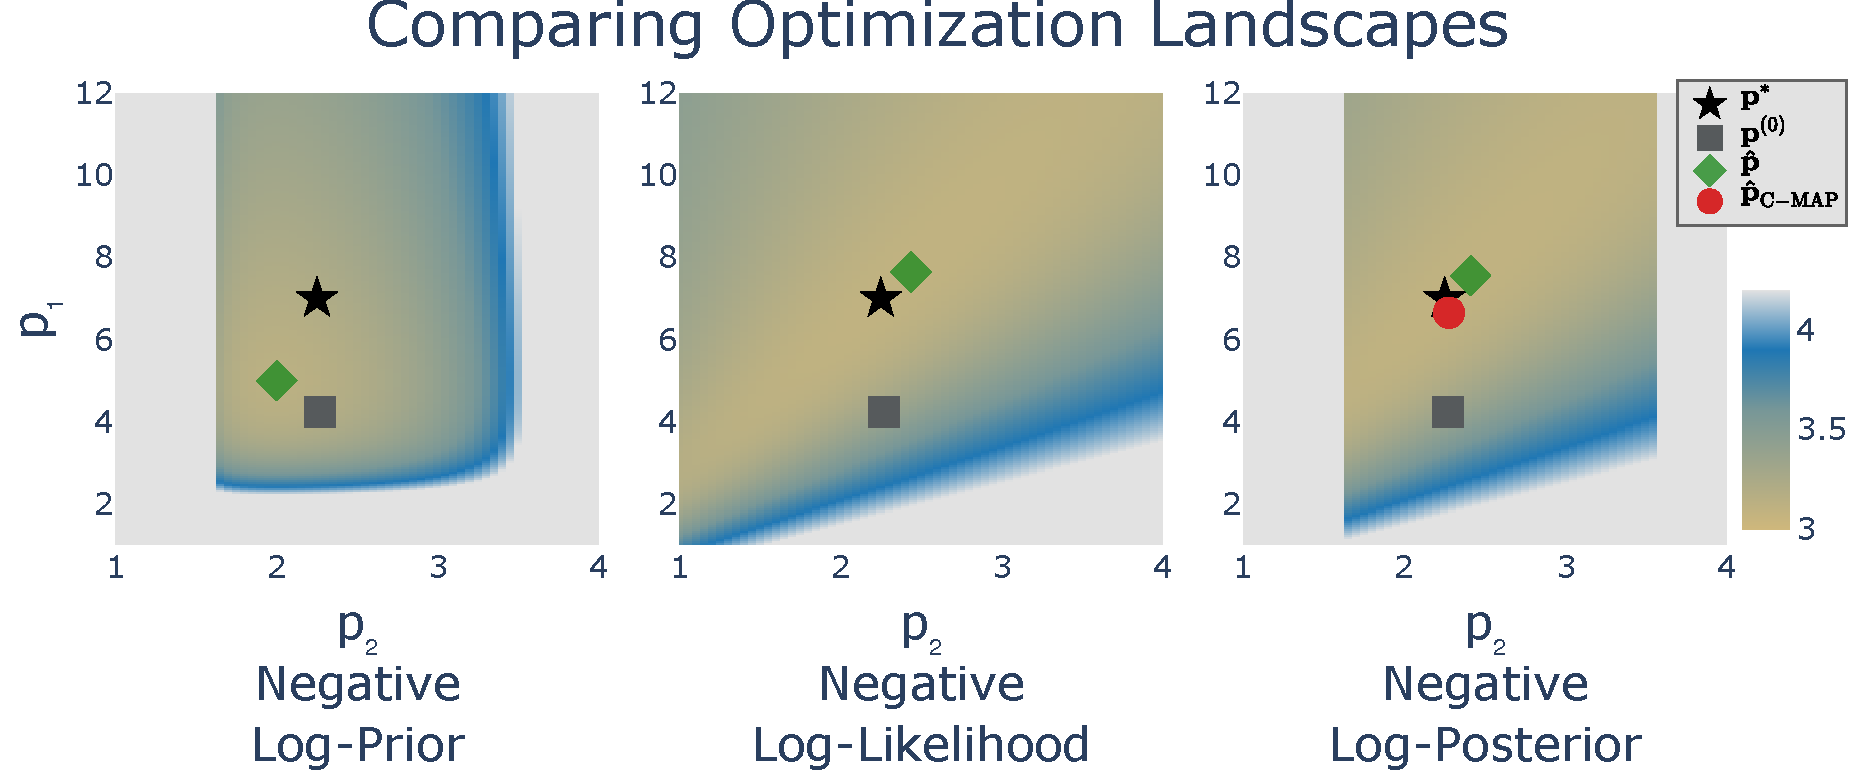
\includegraphics[width=1\linewidth]{figures/LogisticGrowth_OptimizationLandscape.pdf}
        \label{fig:LogisticGrowth_OptimizationLandscape}
    \end{figure}
    Optimizing the prior or the likelihood alone leads to an estimate that is less accurate than either the MAP or its correction.
    % \small
    \begin{table}
    \begin{tabular}{llc}
        \textbf{Objective} && \textbf{Relative Parameter Error}\\
        \midrule
        Prior &$\hat{\p}_{\Pi}$ & 27.4\% \\
        Likelihood &$\hat{\p}_{\mathrm{MLE}}$ & 9.1\% \\
        Posterior &$\phat$ & 7.9\%\\
        Corrected &$\hat{\p}_{\mathrm{cor}}$ & \textbf{4.7\%}\\
        OE-LS & $\hat{\p}_{\mathrm{OE-LS}}$ & 7.3\%
    \end{tabular}
    \end{table}
    \vspace{-.2cm}
\end{exampleblock}


% \begin{exampleblock}{Example: Hindmarsh-Rose}

%     \textbf{Conclusion}: \alert{The WENDy algorithm converges to reasonable parameters more often} than the forward solver based method. 
    
% \end{exampleblock}
\end{column}
\end{columns}
\end{frame}
\end{document}